% Copyright 2019 Clara Eleonore Pavillet

% Author: Clara Eleonore Pavillet
% Description: This is an unofficial Oxford University Beamer Template I made from scratch. Feel free to use it, modify it, share it.
% Version: 1.0

\documentclass{beamer}
\usepackage{pdfpages}
% Load Packages
\usepackage[utf8]{inputenc}
\usepackage{xcolor}
\usepackage{tikz}
\usetikzlibrary{positioning,calc}
\usepackage{graphicx}
\usepackage{hyperref}
\usepackage{amsmath}
\usepackage{listings}
\usepackage{fontawesome}
\usepackage[T2A]{fontenc}
\usepackage[utf8]{inputenc}
\usepackage[russian]{babel}

% Define Commands
\newcommand*{\ClipSep}{0.06cm} %To adjust footer logo
\newcommand{\E}{\mathrm{e}\,} %\def\I{e} % used to defined e for exp(x), see later what it should be
\newcommand{\ud}{\mathrm{d}}
\lstset{numbers=left, numberstyle=\tiny, stepnumber=1,firstnumber=1,breaklines=true,
    numbersep=5pt,language=Python,
    stringstyle=\ttfamily,
    basicstyle=\footnotesize, 
    showstringspaces=false
}

\usetheme{oxonian}
\usepackage{wrapfig}
\usepackage{listings}

\title{Използване на OpenMP - част 5. Sections, flush, threadprivate.}
\subtitle{\textit{Курс „Паралелно програмиране“}}
\titlegraphic{{
\includegraphics[width=5.3cm]{iaps.png}}} 

\author{\newline \newline Стоян Мишев}

\vspace{1cm}

\date{} %\today

\begin{document}
\lstset{language=Python}
{\setbeamertemplate{footline}{} 
\frame{\titlepage}}


\section*{План}\begin{frame}{План}\tableofcontents\end{frame}

%%%%%%%%%%%%%%%%%%%%%%%%%%%%%%%%%%%%%%%%%%%%%%%%%%%
\section{Sections}
\begin{frame}{Sections. Определение.}
  ``\textit{The sections construct is a noniterative worksharing construct that
  contains a set of structured blocks \textbf{that are to be distributed among
  and executed by the threads} in a team. \textbf{Each structured block is
  executed \underline{once} by one of the threads} in the team in the context of
  its implicit task.}''
\end{frame}

\begin{frame}[fragile,fragile]
  \frametitle{Sections}

    \begin{lstlisting}
#pragma omp parallel sections
{
    #pragma omp section
    { 
        printf ("id = %d, \n", omp_get_thread_num());
    }

    #pragma omp section
    { 
        printf ("id = %d, \n", omp_get_thread_num());
    }
}
    \end{lstlisting}
  
\begin{verbatim}
id = 0,
id = 1,
\end{verbatim}

\end{frame}



%%%%%%%%%%%%%%%%%%%%%%%%%%%%%%%%%%%%%%%%%%%%%%%%%%%
\section{flush}
\begin{frame}[fragile]{Flush. Определение.}
  При изпълнението на \verb+flush+, дадена нишка има ``consistent'' достъп до мястото в паметта, описано от \verb+flush set+. \pause
  \centering
  
\includegraphics[width=0.35\textwidth]{flush}
\end{frame}

\begin{frame}
  \frametitle{Flush. Подразбиране}
  \centering
  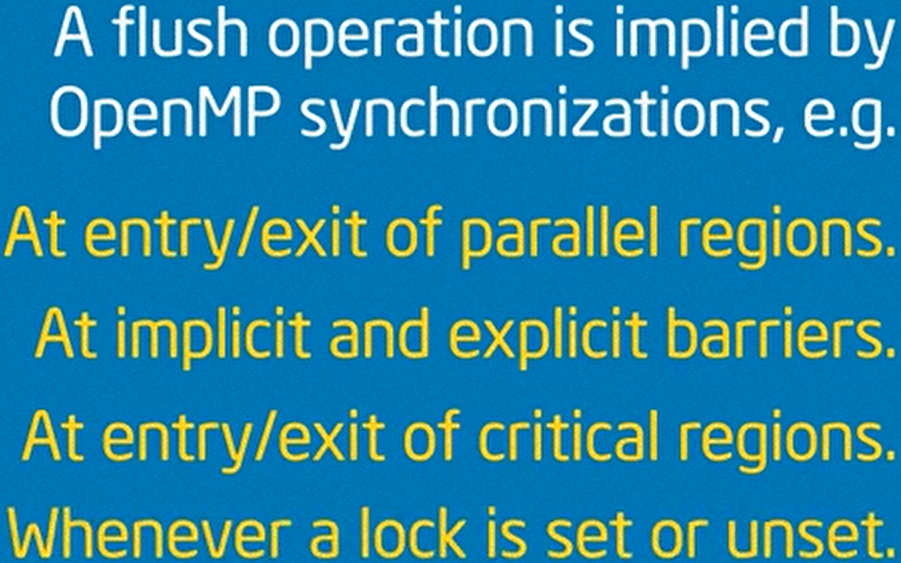
\includegraphics[width=0.45\textwidth]{flush1}  
\end{frame}

\begin{frame}[plain]{Producer-consumer}
  \centering
  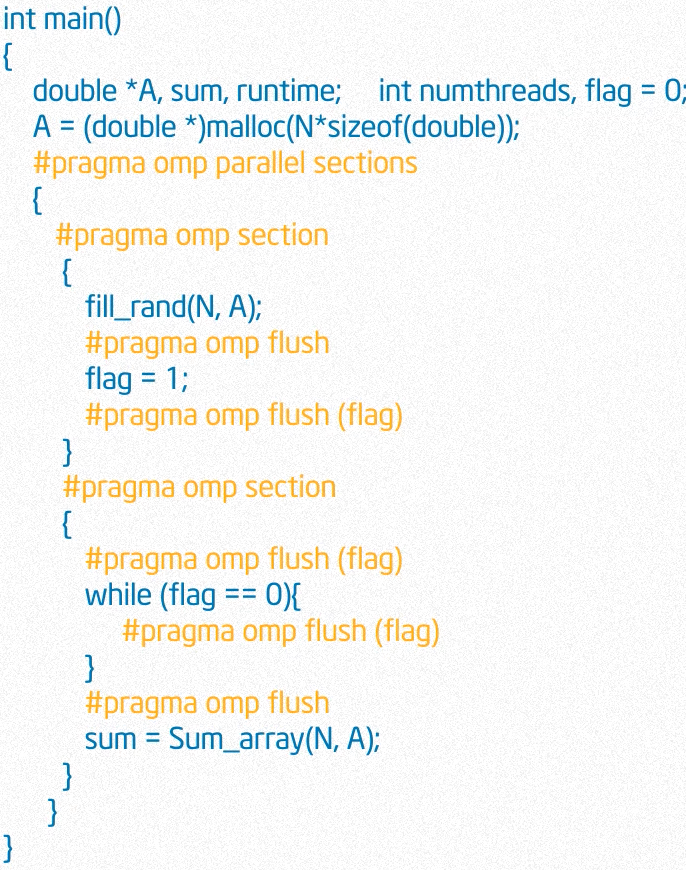
\includegraphics[width=0.59\textwidth]{section-flush}    
\end{frame}

\begin{frame}[plain]{Producer-consumer}
  \centering
  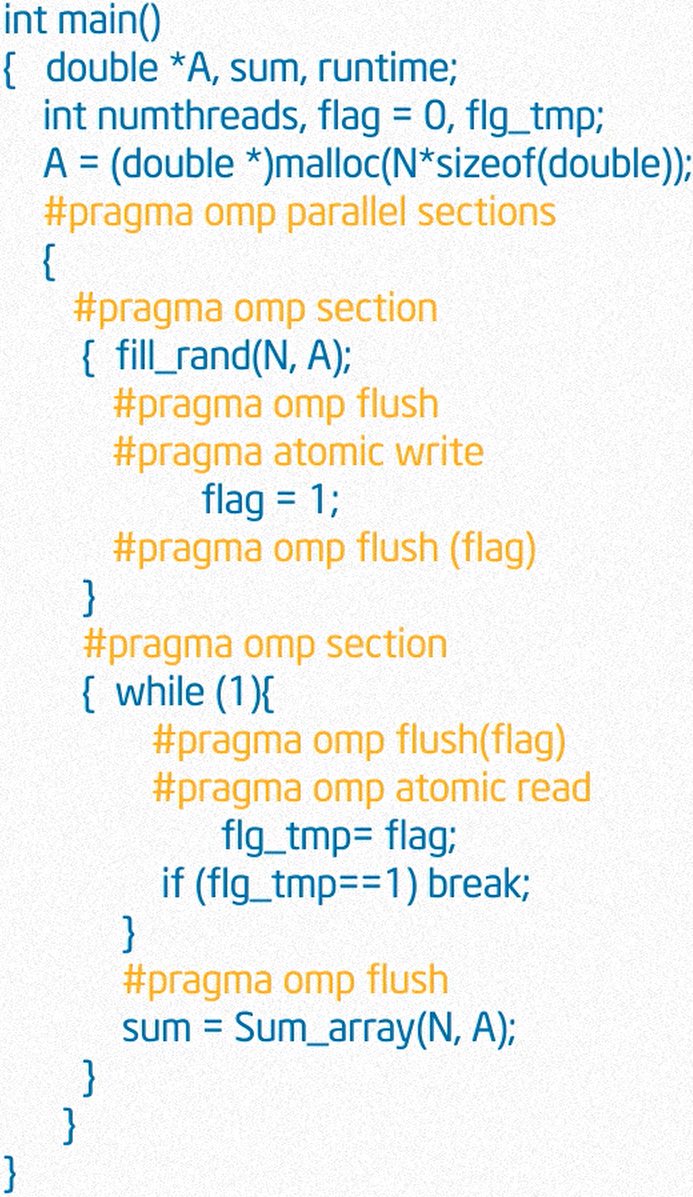
\includegraphics[width=0.45\textwidth]{section-flush1}    
\end{frame}

%%%%%%%%%%%%%%%%%%%%%%%%%%%%%%%%%%%%%%%%%%%%%%%%%%%
\section{threadprivate}
\begin{frame}{threadprivate}
  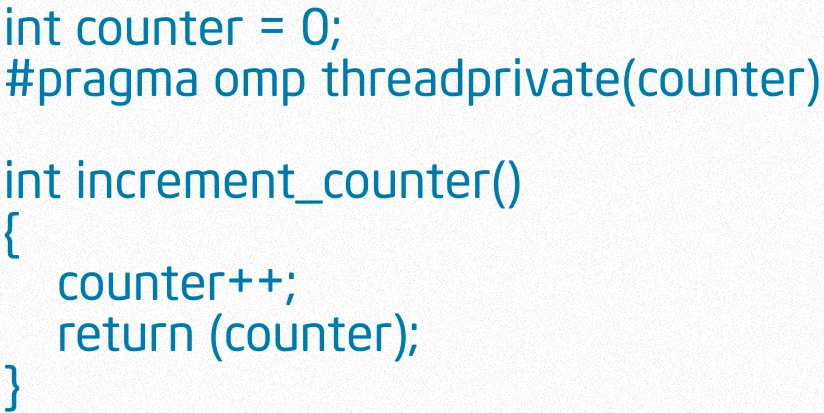
\includegraphics[width=0.45\textwidth]{threadprivate}  
\end{frame}


\begin{frame}
  \frametitle{Домашна работа}
  от \textit{Introduction to OpenMP_ 18 Module 10} до \textit{Introduction to OpenMP_ 21 Discussion 9}

\end{frame}


\end{document}


%%% Local Variables:
%%% mode: latex
%%% TeX-master: t
%%% End:

